%========================================
% Cnot 1.7 — main.tex
%========================================
\documentclass[12pt,oneside,a4paper]{book}

% ---------- Encoding & lingua ----------
\usepackage[T1]{fontenc}
\usepackage[utf8]{inputenc} % con XeLaTeX/LuaLaTeX non serve
\usepackage[italian]{babel}
\usepackage{microtype}

% ---------- Impaginazione ----------
\usepackage[a4paper,margin=2.5cm]{geometry}
\usepackage{setspace}
\onehalfspacing

% ---------- Grafica & colori ----------
\usepackage{graphicx}
\usepackage{xcolor}
\usepackage{float}
\graphicspath{{media/}{figures/}{images/}}

% ---------- Tipografia ----------
\usepackage{csquotes}
\usepackage{booktabs}
\usepackage{array}

% ---------- Riferimenti & PDF ----------
\usepackage{hyperref}
\hypersetup{
  pdftitle={Cnot 1.7},
  pdfauthor={Edizioni Tradizionali},
  pdfsubject={Romanzo / Progetto Cnot 1.7},
  pdfkeywords={Cnot 1.7, narrativa, Edizioni Tradizionali},
  colorlinks=true,
  linkcolor=black,
  citecolor=black,
  urlcolor=black
}
\usepackage{bookmark} % segnalibri robusti

% ---------- Intestazioni/Piè di pagina ----------
\usepackage{fancyhdr}
\pagestyle{fancy}
\fancyhf{}
\fancyhead[LE,RO]{\thepage}
\fancyhead[LO]{\nouppercase{\rightmark}}
\fancyhead[RE]{\nouppercase{\leftmark}}

% ---------- Titoli ----------
\usepackage{titlesec}
\titleformat{\chapter}[display]
  {\bfseries\Huge}
  {\filright\Large\MakeUppercase{\chaptername}\ \thechapter}
  {1ex}
  {\titlerule\vspace{1ex}\filright}
\titlespacing*{\chapter}{0pt}{-2pt}{2.0em}

% ---------- Comandi utili ----------
\newcommand{\CCBYSA}{\includegraphics[height=1.2em]{cc-by-sa.png}} % opzionale

% ---------- Dati del libro ----------
\title{\textbf{Cnot 1.7}}
\author{Edizioni Tradizionali}
\date{\today}

% ---------- (Opzionale) includeonly per compilazioni rapide ----------
% \includeonly{chapters/frontespizio,chapters/premessa,chapters/prologo,chapters/capitolo01}

\begin{document}

%========================================
% Front matter
%========================================
\frontmatter
\maketitle % Se preferisci un frontespizio personalizzato, commenta questa riga e usa chapters/frontespizio.tex

% Frontespizio personalizzato (opzionale, sostituisce \maketitle)
% chapters/frontespizio.tex
\clearpage
\thispagestyle{empty}
\begin{titlepage}
  \centering
  \vspace*{8mm}

  {\Large EDIZIONI TRADIZIONALI\par}

  \vspace{20mm}

  {\Huge\bfseries Cnot~1.7\par} % Titolo
  \vspace{6mm}
  {\Large Eiren Lysias\par}     % Autore

  \vfill

  % Logo (opzionale)
  \includegraphics[width=0.22\linewidth]{media/edizioni tradizionali.png}\par

  \vspace{3mm}
  {\large Ferrara, 2025\par}

  \vspace{8mm}
  {\small
    \textit{“Edizioni Tradizionali” è un \textbf{marchio in fase di registrazione}.\\
    Non è (ancora) una casa editrice; questa è un’\textbf{opera pubblica}.}\par
  }

  \vspace{6mm}
  {\small
    Progetto e sorgenti su GitHub:\par
    \url{https://github.com/francescosisini/Cnot-Franchise}\par
  }

  \vspace{6mm}
  {\small Prima edizione: ottobre 2025 \quad\textbullet\quad ISBN: \textit{da assegnare}\par}

\end{titlepage}
\clearpage


% Indice (se lo vuoi all’inizio)
\tableofcontents
\cleardoublepage

% Premessa (non numerata ma in front matter)
% chapters/premessa.tex
\cleardoublepage
\chapter*{Premessa}
\markboth{Premessa}{Premessa}

\section*{Nota sull'universo narrativo}
\textit{Cnot 1.7} fa parte dell’universo narrativo \textbf{Cnot}, ideato e sviluppato da Francesco Sisini.
Il progetto comprende anche il romanzo \textit{Cnot}, che introduce le protagoniste e i temi scientifici, etici e ambientali alla base della saga.
Ogni volume è indipendente, ma insieme formano un percorso sulla mente, la tecnologia e la responsabilità verso la Terra. %

\section*{Note sul luogo}
Il convitto descritto nel romanzo è ispirato a una vera struttura sanitaria dismessa, situata in un’area urbana quasi identica a quella riportata nelle mappe.
Ogni riferimento topografico è trattato con rispetto per la memoria dei luoghi e per la storia delle persone che li hanno abitati. %

\section*{Ringraziamenti}
A chi crede che la scienza e la narrativa possano parlarsi senza tradirsi.
A chi osserva il mondo con curiosità, anche quando sembra fermo.
E a chi riconosce, nei fili della tecnologia, un’estensione della vita stessa. %

\vspace{2em}
\begin{center}
\footnotesize
Impaginato in HTML e PDF con strumenti open-source.\\
\textcopyright\ Francesco Sisini, 2025 — Alcuni diritti sono riservati CC BY-SA.
\end{center}


% Prologo (puoi decidere se tenerlo in frontmatter o passare a mainmatter prima)
% chapters/prologo.tex
\cleardoublepage
\chapter*{Prologo. Lacrime in cameretta}
\markboth{Prologo}{Prologo}

Alice è arrabbiata, risentita, offesa, triste e amareggiata, per questo le lacrime le stanno rigando gli occhi.
Soffre, ma non darà a sua madre la soddisfazione di vederla così.
Resta chiusa in camera, al riparo senza che nessuno possa vedere, minimizzare, giudicare.
Prende un quaderno, una penna e la chitarra che le ha regalato suo padre dopo il saggio di flauto: «Ora impara con questa» le aveva detto. %

Non l'ha studiata molto, ma conosce gli accordi principali e, nonostante i tempi, sa come si scrive una canzone.
Non solo: sa come si scrive un testo; non uno di quelli più o meno scontati che si trovano in streaming, ma un testo che sa parlare a una sola persona, che sa avvicinarla con delicatezza, farle aprire le porte del cuore per poi piantarci un coltello. %
Già, proprio come ha fatto Caterina con lei.

\begin{figure}[H]
  \centering
  \includegraphics[width=.35\linewidth]{diario alice senza sfondo.png}
  %\caption*{\footnotesize Le parole della canzone sul quaderno di Alice, con accordi per la chitarra.}
\end{figure}

Questa qua sotto è Alice, quasi grande ma ancora adolescente; a vederla nel suo vestitino skater non sembra capace di parole così taglienti.

\begin{figure}[H]
  \centering
  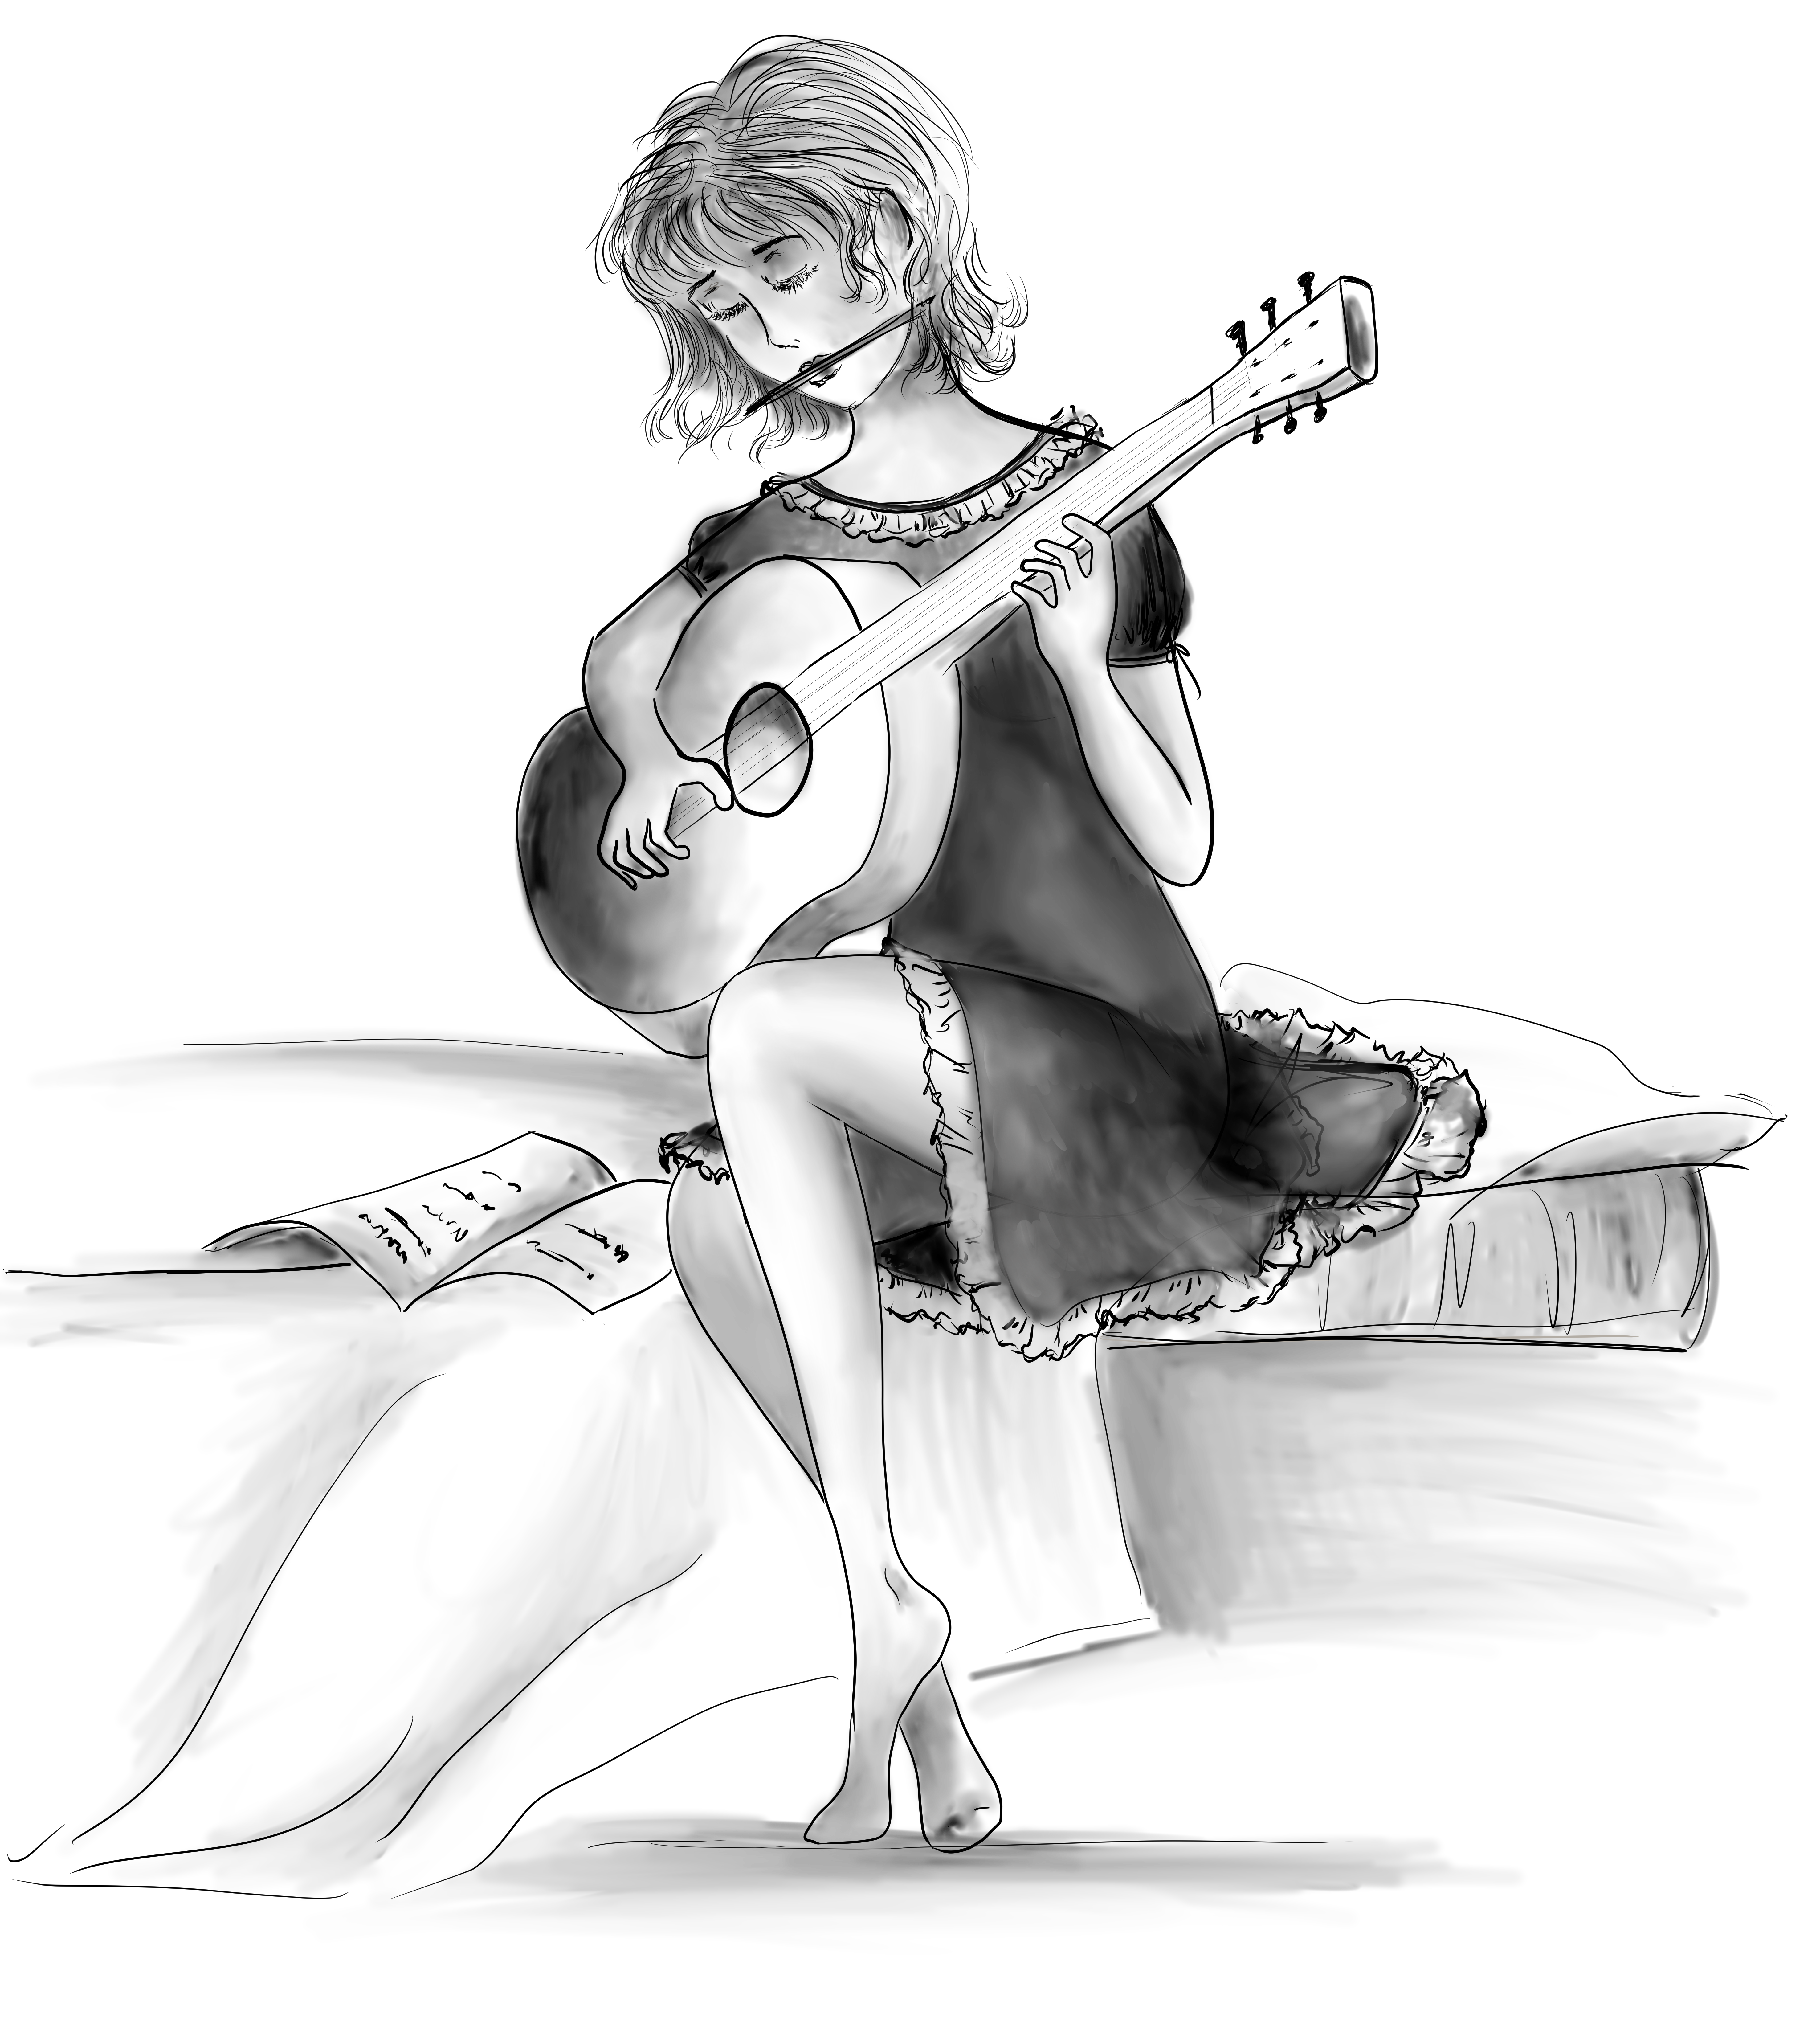
\includegraphics[width=.35\linewidth]{alice senza sfondo.png}
  %\caption*{\footnotesize Alice piange mentre suona la sua canzone.}
\end{figure}


%========================================
% Corpo del libro
%========================================
\mainmatter

% --- 17 capitoli ---
\chapter{Vendetta in SOL maggiore}

Una lettera è un messaggio scritto di pugno e consegnato nella buchetta di casa per mezzo di un servizio postale.  
Oggi lo si usa poco ma per molte persone ha un significato simbolico, indica l'appartenenza al gruppo di chi non ha dimenticato l'origine terrestre degli esseri umani.  
Inizialmente c'era un po' di diffidenza da parte dei più integralisti, ma poi la percezione che la natura è una e ogni albero vive anche nel complesso dell'intera foresta ha spostato le sensibilità verso una posizione più sostenibile, così in molti si sono convinti che la carta non è il male del mondo ed esprimono con le parole il loro dolore per il pianeta che soffre scrivendole con la matita, sulla carta.  
Una matita fatta di legno sulla carta di cellulosa.  
Parole che sanno di albero che vengono spedite a destinatari incaricati di caricarsi il peso dell'angoscia.

\par\medskip
Laura è seduta sulla poltroncina degli ospiti che sta aiutando l’amica a sbrigare un po’ della corrispondenza, visto che lei è impegnata in faccende che la coinvolgono molto di più.

\par\medskip
\begin{center}
  \includegraphics[width=.55\linewidth]{image1.png}
\end{center}

\begin{verse}\itshape
«Cara Caterina,\\
ti scrivo con le mani sporche di terra e il cuore in fiamme.\\
Ogni giorno mi sveglio con l’ansia che il cielo sia un po’ più basso,\\
che il vento porti con sé un alto grido soffocato di una specie che non c’è più.\\
Eppure continuo a lottare, perché se ci sei tu,\\
tu che hai il coraggio che io non ho…»
\end{verse}

«Vuoi che continui, Cate? Non mi sembra giunga nulla di nuovo alla discussione…»

«Ma sì dai, mi sembra così angosciata, poverina…»

\par\medskip
Caterina è a pochi decimetri da Laura, davanti all’armadio.

\par\medskip
\begin{center}
  \includegraphics[width=.6\linewidth]{image3.png}
\end{center}

Caterina è proprio lì davanti che sceglie i vestiti da mettere in valigia.

Laura riprende, ma il settanta per cento di ciò che legge le sfugge, perché la sua attenzione è catturata dai movimenti mimetici di Alice, seduta sul letto di fronte a lei.

Un viaggio difficile da organizzare, tra biglietti introvabili, alberghi al completo, impegni precedenti e consegne da rispettare sul lavoro.  
Mancano trentasei ore al volo che la condurrà negli Stati Uniti ed è quasi tutto a posto, ma Caterina non sa che sua sorella le sta cucinando una bella vendetta da gustare calda anziché fredda.

Lei se ne va a New York e la lascia a casa con suo padre e sua madre, proprio ora che potrebbero passare una settimana insieme.  
Certo, Alice comprende che il lavoro è importante. Infatti, se fosse solo per quello, non le brucerebbe così tanto.

Ma il problema non è il lavoro. In realtà, lei ci va per Mark.  
Figurati, se non ci fosse lui, avrebbe sicuramente preferito passare l’estate con lei.  
In fondo, di corsi di aggiornamento ce ne sono tanti, nel mondo.  
No, lei lo sa che è per Mark.

\par\medskip
Così, tranquilla, con il suo PC in mano, a gambe incrociate sul letto, mostra uno sguardo innocente.

Vediamo di vedere dove è seduta. Disegniamo anche il letto e, visto che ci siamo, anche la scrivania.  
Dalla camera di una ragazza si può capire molto di lei:

\par\medskip
\begin{center}
  \includegraphics[width=.6\linewidth]{image2.png}
\end{center}

Eccola qui.  
Uno spazio ampio al centro con i mobili accostati verso le pareti, Caterina preferisce l'essere all'apparire.  
La stanza ha tre poli, come i quark: uno per il lavoro, uno per il relax e uno per riposare.  
Che carina, è proprio ordinata.

\par\medskip
Ma torniamo ad Alice.  
Laura le si avvicina per sbirciare cosa sta facendo, ma Alice, con una piccola rotazione, si sottrae al suo sguardo.

«Scusami, sai!» la rimprovera dell'indiscrezione.  
Poi incolla il testo nella sezione \textit{Lyrics} di Suno:

\par\medskip
\textbf{Lyrics}
\begin{quote}\itshape
She leaves and I stay\\
like a folder left open\\
half full, half erased\\
I blink, and she’s already gone
\end{quote}

«Qui capirai quanto ci sono rimasta male…»

\par\medskip
\textbf{Style Description}
\begin{quote}\itshape
Bilingual emotional synth-pop with ambient textures, cinematic flow, and AI female vocals.\\
Slow build. Glitchy, dreamlike, bittersweet. Like diary pages sung in code.
\end{quote}

«Lascia da perdere, è arrabbiata con me.»

«Non sono arrabbiata, solo che voglio finire una cosa.»

«Ha ragione, sono io che sono troppo curiosa.  
Però si è fatta un po’ tardi, è ora che vado a prendere Valentina.»

«No, aspetta solo un attimo, ti prego.»

«Ora la scarico, colleghiamo le casse e voilà!»

\par\medskip
Le note di pianoforte sintetico arpeggiano velocemente una nenia in Sol maggiore.  
Poi, con un respiro sussurrato, inizia il primo verso:

\par\medskip
\textbf{Verse 1}
\begin{quote}\itshape
She leaves and I stay\\
like a folder left open\\
half full, half erased\\
I blink, and she’s already gone
\end{quote}

Questa è la scena prima della crisi…

\par\medskip
\begin{center}
  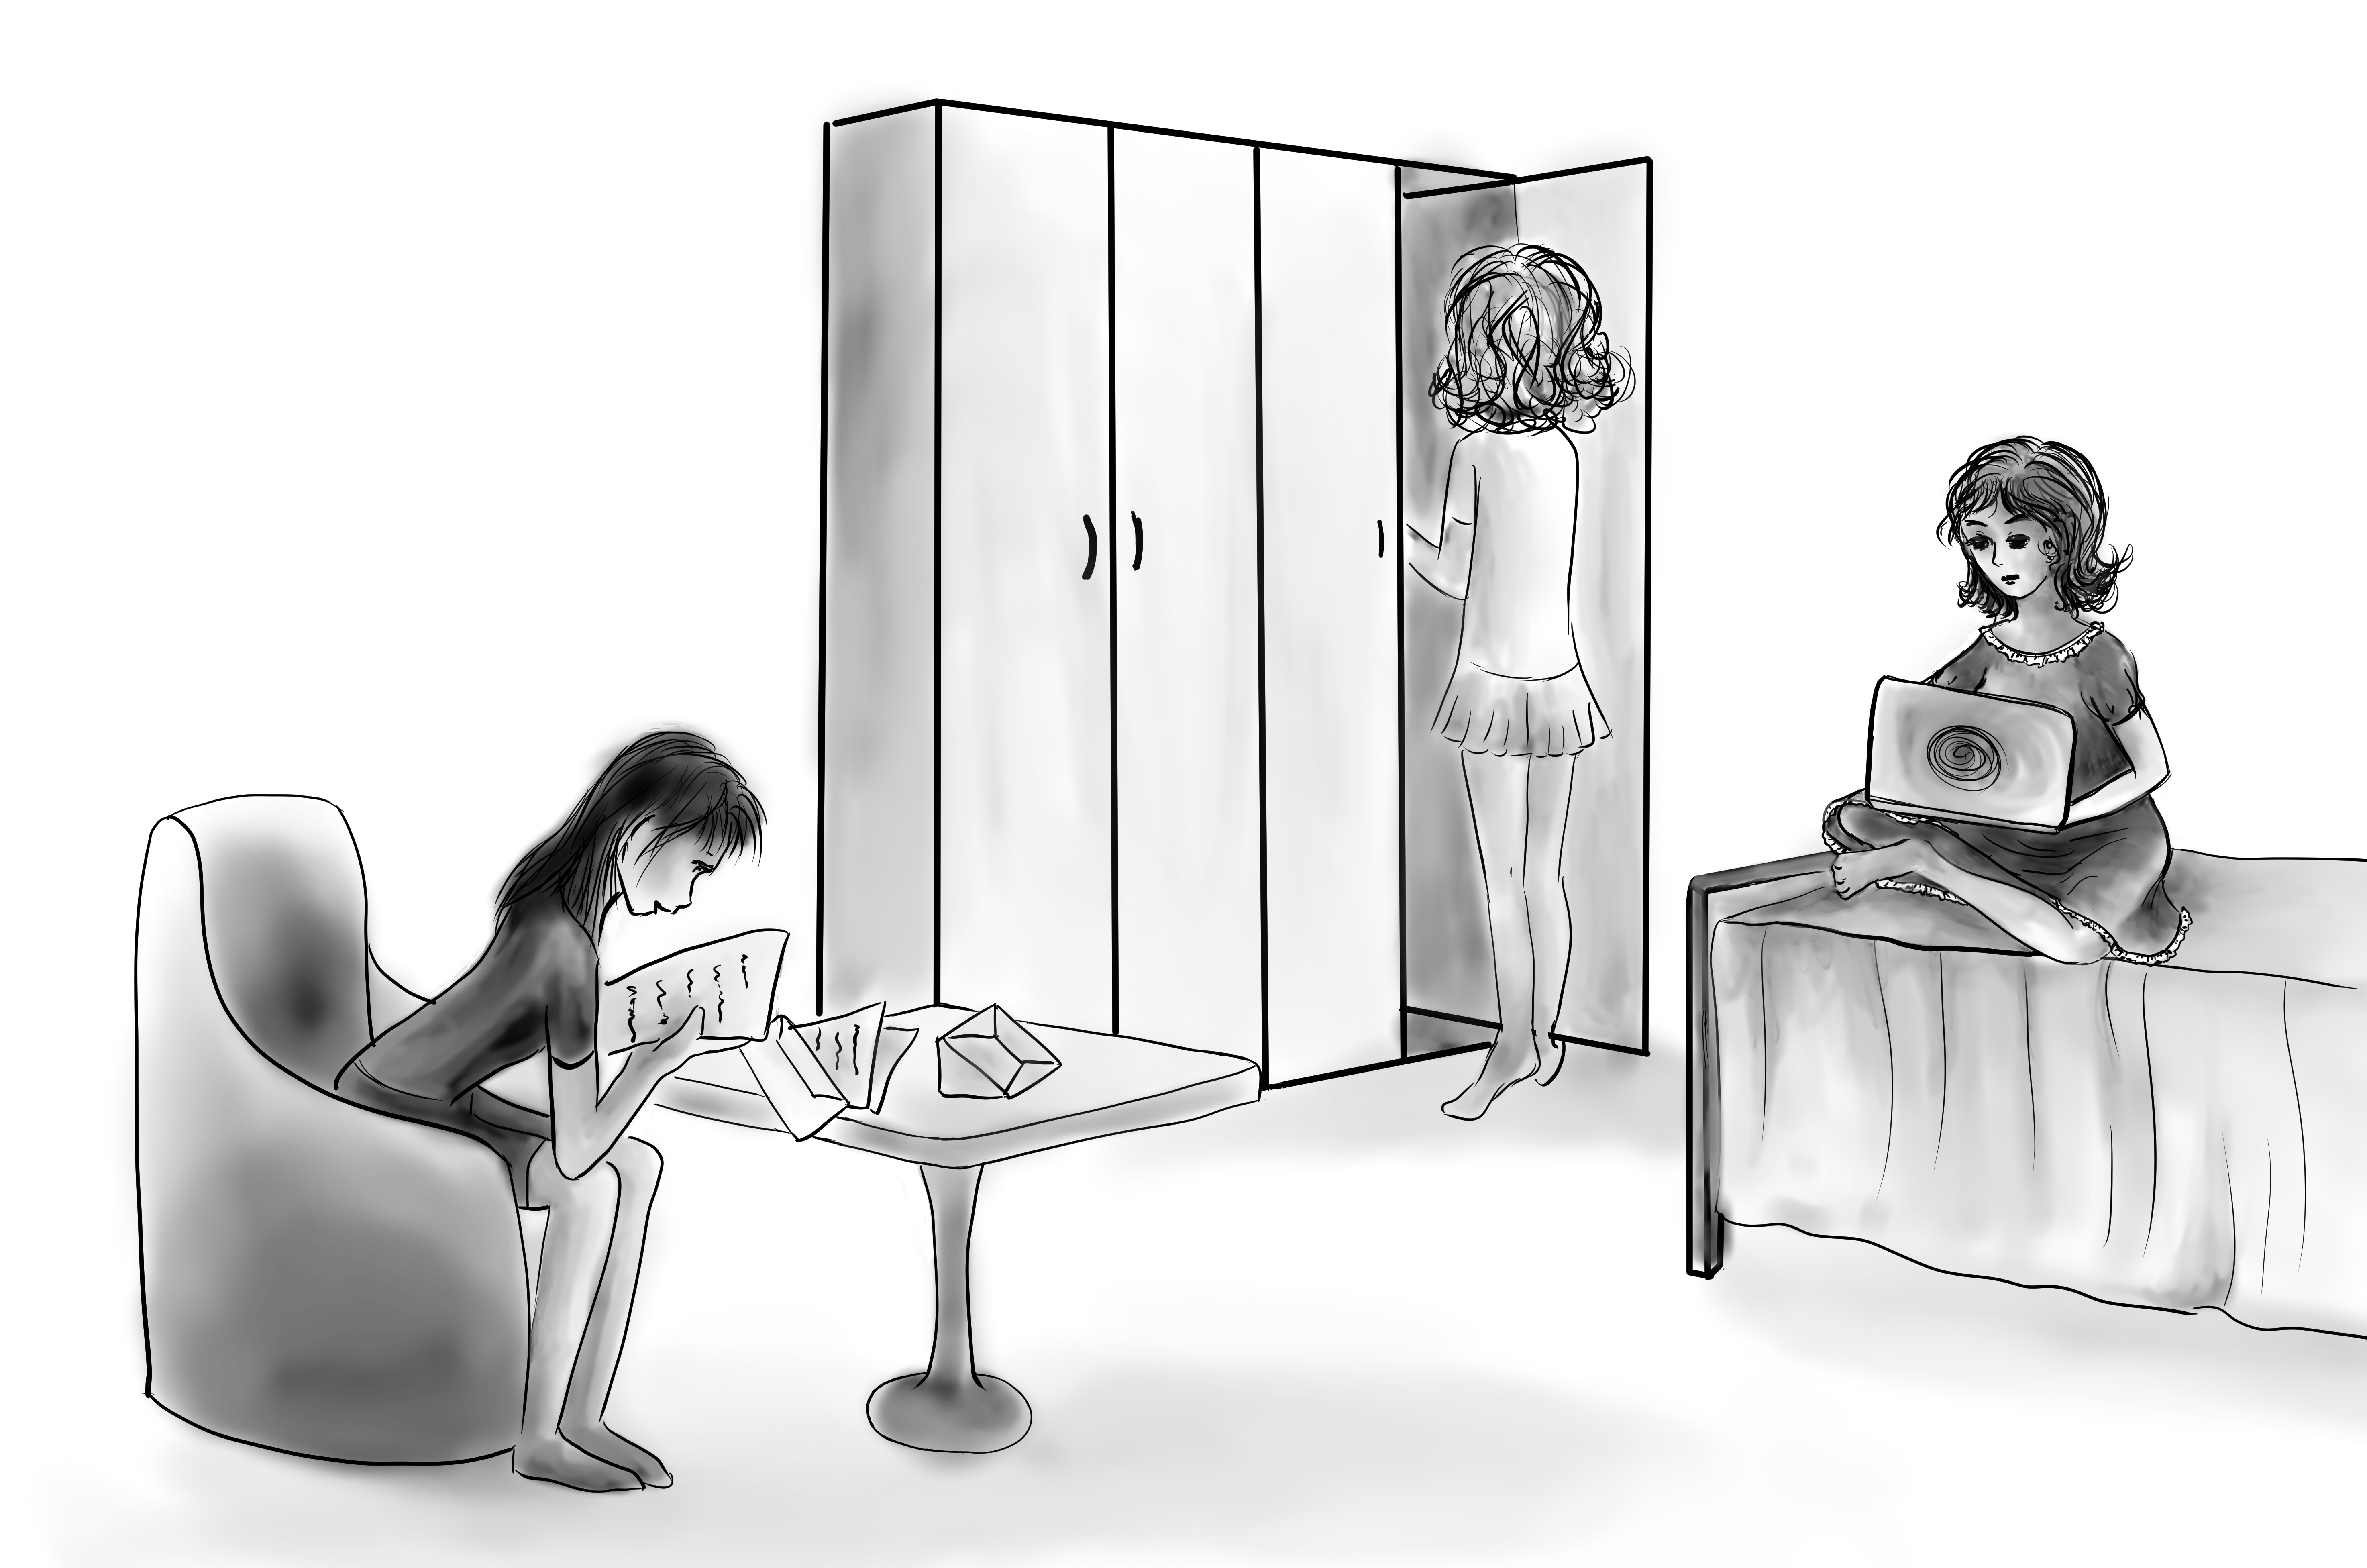
\includegraphics[width=.6\linewidth]{ccsf.png}
\end{center}

\textbf{Verse 2}
\begin{quote}\itshape
She goes to New York\\
I stay with a lamp shaped like a heart\\
plastic love, three settings\\
warm, cold, ambient — mine is blinking
\end{quote}

«E qui voglio vederti piangere!»

\begin{quote}\itshape
I'm not angry, I'm just here
\end{quote}

Una lacrima solca il viso di Caterina, che a stento simula tranquillità continuando a ordinare le cose da mettere in valigia.

«Certo che le semplifichi proprio la partenza, tu.»

Caterina appoggia l’asciugacapelli e si avvicina alla sorella per abbracciarla.

«Non ci provare!» le urla.

Caterina non reagisce. È abituata.  
Alice si libera le ginocchia dal PC e lo poggia sul letto.

«Io esco, mangio qualcosa con le ragazze.»

Caterina si asciuga gli occhi.

«Va bene, ma a casa per le dieci. È l’ultima sera che passiamo insieme.»

«Devo andare anch’io, Cate.»

«Va bene Laura, grazie di essere venuta.»

«Ciao Cate. Ciao Alice.»

Prima di chiudere la porta, Laura ha un attimo di esitazione.  
C’era ancora una cosa, anzi, il motivo principale per cui aveva raggiunto Caterina.

«Ma non sai ancora nulla del visto!»

«Non preoccuparti, Laura. Vedrai che non ci saranno problemi.  
In ogni caso, se ci fossero difficoltà ti chiamo.»

Saluta l’amica con un bacio e corre a prendere Vale.  
Per fortuna manca ancora qualche anno alla sua adolescenza.

\include{chapters/chapter02}
\chapter{Il ricorso}

«Cosa prepari per cena?»\\
«Tu cosa avresti voglia di mangiare?»

\par\medskip
\begin{center}
  \includegraphics[width=.7\linewidth]{soggiorno_tiny.png}%
\end{center}

«I bastoncini fritti? Prepari i bastoncini fritti?»\\
«Infatti.»\\
«Davvero ci sono i bastoncini?»\\
«No, c’è il riso integrale con le verdure.»\\
«Perché sempre le verdure?»\\
«Perché ce ne abbiamo nell’orto, sono buone e fanno bene.»\\
«Ma io ho voglia di bastoncini. Quando li mangiamo?»\\
«Venerdì. A fine settimana vado a fare la spesa.»

Rocky abbaia e si avvicina alla porta. Laura non finisce la frase e dalla vetrata intravede Caterina che sta arrivando.

«Guarda, arriva Caterina. Non farle vedere che fai i capricci.»

Caterina raggiunge la pedana antistante la vetrata, ma non fa in tempo a entrare che una distesa di matite e colori le occupa il tappeto davanti all’entrata. Caterina non entra subito. Penne, pennarelli, lapis, fogli di album da disegno le sbarrano la strada. Valentina si alza e la trascina dentro, con un piccolo salto sopra la distesa.

\par\medskip
\begin{center}
  \includegraphics[width=\linewidth]{soggiorno_prospettiva.png}%
\end{center}

«Stai facendo i compiti?»\\
«Anche, ma non solo. Stavo disegnando la terra di Hokuto.»\\
«La terra di Hokuto? E dove si trova?»\\
«In Giappone, dopo la Cina.»

Caterina si inginocchia su un cuscino accanto a Valentina.

«Vedi, qui è dove si trova la scuola di Hokuto.»

Caterina si avvicina al disegno.

«Sì? C’è anche un maestro?»\\
«Certo, è il padre di tre fratelli…>»

«Vale, forse Caterina doveva dirmi qualcosa…»

«Lascia che mi racconti Laura. È passato tanto tempo da quando Alice non mi mostra più i suoi disegni…»

«Anche Alice fa i disegni? Me li porti?»

«Li faceva da piccola tesoro, adesso mi scrive le canzoni….»

«Che bello, le voglio ascoltare!»

Caterina le sorride e appoggia il disegno sul tavolo.

«Mi hanno negato il visto, Laura. Ho tempo fino alle ventiquattro per fare ricorso.»

Laura appoggia il coltello sul tagliere e guarda verso l’amica.

«Quando l’hai saputo?»\\
«Due ore fa eri a casa mia e non lo sapevo ancora... quindi?»\\
«Hai ragione, Cate, scusami.»\\
«No, scusami tu. Sono stata acida. È che sono disperata.»\\
«Ma hai già sentito Mark?»\\
«Sì, è stato lui a dirmi della possibilità di fare ricorso.»\\
«Oh, Laura, come facciamo?»

Laura si avvicina e la prende per le braccia.

«Cate, ne abbiamo passate di peggio.»\\
«Però, se il tempo stringe, vediamo prima il ricorso, poi apparecchiamo.»

Non finisce la frase che il brontolio della pancia di Valentina rompe l’attenzione che si era creata.

«Non ceniamo?»\\
«Ceniamo?»\\
«Tra poco, Vale.»

Laura prende il portatile dalla cameretta insieme a un tavolino pieghevole. Le due amiche si siedono accanto a Valentina.

«Vediamo come funziona il ricorso.»

Caterina accenna un sorriso, ma la voce le trema: «Ho tempo fino a mezzanotte.»

Laura la fissa per un istante, poi abbassa lo sguardo sullo schermo.

«E Mark… ti ha detto tutto del suo lavoro?»\\
«Credo… di sì… perché?»

Laura inspira piano. «Perché forse qualcuno non ti vuole lì.»

\chapter{Il ritorno di Ipparchia}

«Ippa! Ippa! Ipparchia!»\\
La sta chiamando forte, ma ancora non torna. Giovanni si siede sul muretto.

Dietro di lui, un edificio in rovina che non conosce perchè non ne ha ancora esplorato i dintorni. Giovanni ha tempo e lo usa come crede. Ora deve usarlo per attendere Ipparchia. Tiene il cartone sulle ginocchia.

Schopenhauer, ”L’arte di ottenere ragione”, stratagemma numero uno. Lo ripete tutto. Sa che sono passati circa trenta secondi. Se fosse stato un matematico, avrebbe contato, ma non era la matematica la sua passione.\\
Arriva allo stratagemma trentotto, è passato un’ora, e Ipparchia non è ancora tornata.

Dietro di lui, un luogo ignoto. Alla sua destra, la strada per il supermercato; a sinistra, la strada verso casa. Davanti, una via semi-inesplorata, ma la più probabile per ritrovare la cagnetta. Si incammina in quella direzione, continuando a chiamarla.

La strada diventa bianca: l’asfalto finisce, inizia la terra battuta. Da entrambi i lati, lo stesso fruscio tra gli alberi. Ogni quindici metri, un tronco più grande degli altri.

Quando Ipparchia lo ha lasciato erano circa le otto di sera, quindi ora è quasi buio. Per lui non cambia molto, ma i cani usano anche la vista.\\
Arriva a un incrocio: la strada bianca curva a destra, mentre dritto torna asfaltata.\\
«Ippa! Dove sei andata?»

Giovanni tiene la destra e si addentra in campagna. Gli alberi continuano a costeggiare la strada, ne conta nove, poi all’improvviso l’asfalto ritorna.

\par\medskip
\begin{center}
  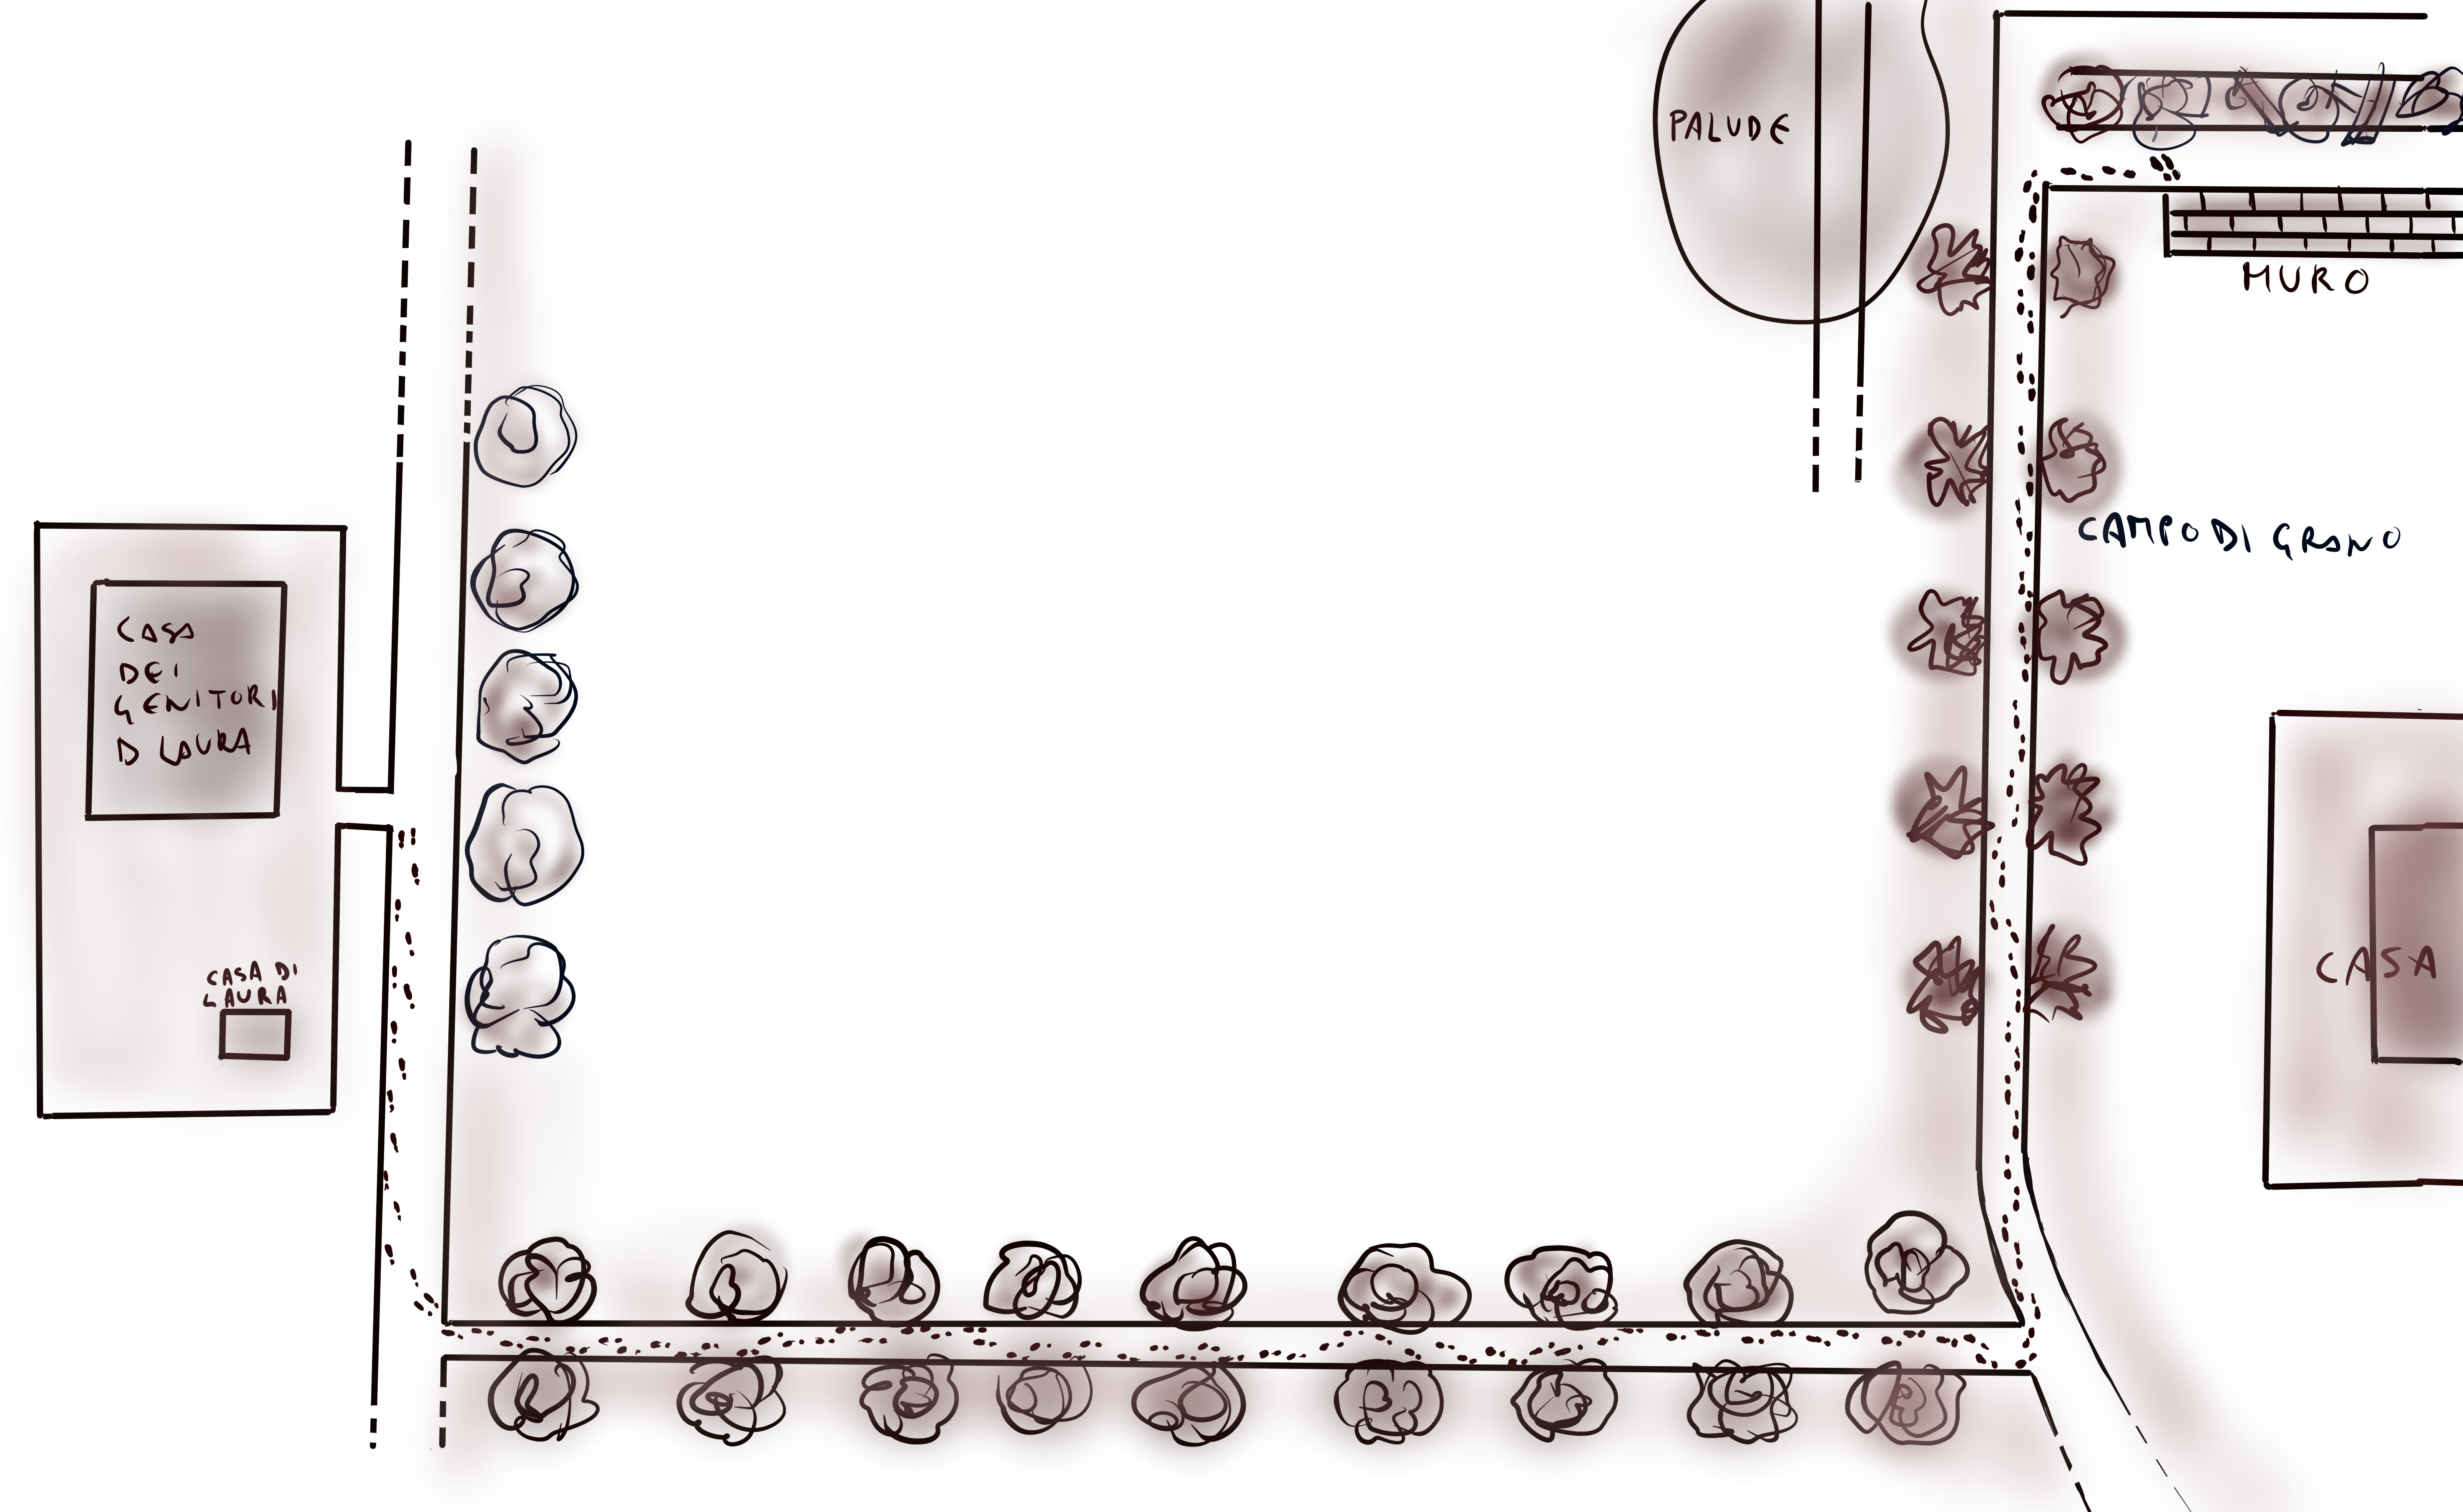
\includegraphics[width=0.9\linewidth]{mappa con casa laura.png}
\end{center}

Attende qualche minuto. Sente passare un veicolo. La strada che ha incontrato taglia quella bianca: deve essere una vecchia via di comunicazione.

Sta per tornare indietro, quando dall’altra parte della strada una voce familiare lo fa voltare:\\
«Ippa!»\\
Attraversa senza esitazione.\\
«Ippa!» Le va incontro, lei rimane ferma, la raggiunge e capisce cosa è successo: il guinzaglio di corda è rimasto incastrato in qualche anfratto, ma Giovanni la libera facilmente.

Ipparchia lo lecca, ma… sono due le lingue. Un altro cane è accanto a lei.\\
«C’è un altro cane qui...» chiama più volte: «C’è un cane qui! E’ di qualcuno questo cane?»\\
Nessuna risposta.

«Andiamo, Ippa.»\\
Ripartono e sul tratto asfaltato il rumore è quello di otto zampe.\\
Raggiungono di nuovo la strada bianca. Giovanni si inginocchia e accarezza il nuovo arrivato.\\
«E tu? Ci segui?» Si gratta la testa. «In ogni caso, non saprei come altro aiutarti per ora. Va bene, andiamo a casa, poi vedremo.»

Ripercorre la strada dell’andata, passo dopo passo, rumore dopo rumore, odore dopo odore.\\
«Coraggio, è tardi, ma si va a cena.»

Giovanni regge il pacco per le ultime decine di metri che lo separano dal rifugio.\\
L’odore delle rose dell’ultima abitazione si mescola alla lavanda spontanea che cresce nel parco abbandonato dell’ex convitto.\\
Avanza tra spine di more e ciuffi di rosmarino, che pungono le gambe e coprono l’odore di Ippa e dell’altro cane. Un dedalo verde che è la sua protezione segreta.

Le braccia gli pesano, ma ormai ce l’ha fatta.\\
Un ramo si spezza a pochi metri:\\
«Ehi, c’è qualcuno?»\\
Silenzio. Nulla di strano, forse solo un ramo secco.

Manca solo da salire la scala antincendio quando, alle sue spalle, una voce lo ferma:\\
«…Appoggia il pacco, amico.»

Giovanni resta immobile.\\
«Mi hai trovato.» Lo dice lentamente, a sentirlo sembrerebbe il copione di un film, tipo Sergio Leone.\\
Lentamente, posa il pacco sul primo pianerottolo e impercettibilmente lascia scorrere la mano verso il fianco.\\
«Io non lo farei…» la voce è leggermente coperta da Ipparchia e il nuovo compagno che ringhiano sommessamente, il pelo irto, lo sguardo fisso verso il buio alle sue spalle.\\
«Tu non sei me, perchè tu sei…»

Un passo nel buio. Qualcosa striscia tra le foglie secche, appena oltre il cerchio di luce.

Giovanni stringe le mascelle.

Ipparchia e l’altro cane ringhiano più forte, le zampe piantate a terra.

Poi la voce, ferma e bassa:

«… un uomo morto.»

Un colpo secco, come di legno che batte sul metallo, rompe il silenzio.

% chapters/chapter05.tex
\chapter{Che lavoro fa Mark?}

La domanda l'ha spiazzata e l'ipotesi di Laura ancora di più. Rimane attonita a guardare l'amica.

\par\medskip
«Vale vai a lavarti le mani, è pronto»\\
\par\medskip
«Deve venire anche Caterina però!»\\
\par\medskip
«Vai pure Cate, ne parliamo dopo cena, ma credo di aver capito il problema, e forse ho un’idea per sbloccare la situazione. Però ora mangiamo, le abitudini sono fondamentali per Valentina…»\\
«Vado a lavarmi le mani.»

\par\medskip
Hanno finito di mangiare: Rocky dorme ai piedi di Cate sazio di quanto gli è stato passato. Brutta abitudine dare da mangiare ai pulciosi da tavola, difficilmente vi rinunceranno!\\
Laura si alza per sparecchiare, Valentina scappa sul tappeto per finire i suoi disegni, mentre lo sguardo di Caterina torna serio e preoccupato:

\par\medskip
«Lo sapevo che il lavoro di Mark prima o poi mi avrebbe ostacolato!»

\par\medskip
«È probabile che la compagnia pretenda controlli stretti sui parenti. Non possono rischiare: tu hai già manifestato contro di loro.»

\par\medskip
«È il colmo. Non posso andare a New York perché il mio fidanzato lavora per una compagnia che detta le strategie energetiche. Quindi la mia libertà dipende dai miei affetti? Come posso accettarlo, Laura?»\\
«Cate…»\\
«no, scusami, tu non c’entri.»\\
«Cate, posso fare un paio di telefonate»\\
«Ma Laura, non volevo…»\\
«Non preoccuparti. Ora però lasciami da sola, metto a letto Vale e me ne occupo.»\\
«Sì, vado. Ormai deve tornare anche Alice.»\\
«Mi fai sapere?»\\
«Sì, tranquilla. Ti accompagno.»

\par\medskip
Laura e Caterina escono sulla pedana e raggiungono il prato.\\
«Fa fresco…»\\
«Mi sa che hai lasciato la giacca in casa. Te la porto.»

\par\medskip
Caterina rimane sola. Alza lo sguardo verso le stelle.\\
«Eccolo, Cate.»\\
«Grazie.»\\
«Allora, mi aggiorni?»\\
«Certo.»

\par\medskip
Caterina si dirige verso casa mentre Laura guarda l’amica diventare una luce nel firmamento.

\par\medskip
«Andiamo a letto!»\\
La voce di Valentina la raggiunge. La sente forte.

\par\medskip
Rientra. Valentina si è già lavata i denti e ha steso i due futon in camera.\\
«Hai proprio sonno?»\\
«No, è che voglio la storia. Dai, leggiamo!»\\
«Ma… ok, però solo un capitolo, perché poi devo fare una cosa per Cate.»\\
«Cosa devi fare?»\\
«Una cosa da grandi. Meglio se non te la dico, sennò poi dovrei tagliarti la lingua!»

\par\medskip
Valentina ride. Laura prende il manga dalla libreria in sala e si sdraia sul futon vicino a lei.\\
Raggiungono il segno dove erano arrivate a leggere la sera prima. Vale appoggia la testa sulle spalle di Laura, che comincia a leggere le nuvolette.

\par\medskip
Scorrono cinque pagine, poi Vale sbadiglia.\\
«Hai sonno? Non finiamo il capitolo?»\\
«È lo stesso, adesso dormo. Tu cosa fai?»

\par\medskip
«Devo fare quella cosa per Caterina»\\
«Posso venire con te?»\\
«Ma non hai detto che hai sonno»\\
«Si, ma voglio vedere che…»

\par\medskip
Valentina non finisce la frase, ha davvero sonno. Comunque Laura è abituata a vederla crollare di sera, d’altra parte anche se non è una psicologa conosce gli effetti della perdita anche su sé stessa.\\
Lascia la porta della loro stanza socchiusa. Prende la caraffa di tè freddo dal frigo e lo versa in un bicchiere di vetro grosso di color arancione. Dal credenzino sotto la libreria prende il DPL, un dispositivo di programmazione con kernel Linux. Non farà telefonate, forzerà il server della polizia municipale e cancellerà solo qualche dato, senza fare danni. Un’azione discutibile ma efficace.\\
«Vediamo la situazione»

\par\medskip
Laura schizza la rete: i dati di Cate devono svanire dal server giusto un attimo prima che il DHS, via TECS, chieda l’accesso. Poi tornano, invisibili come se nulla fosse.

\par\medskip
\begin{center}
  \includegraphics[width=.9\linewidth]{rete senza sfondo.png}
\end{center}

\par\medskip
«Abbiamo 128 minuti per mappare l'infrastruttura e segnare i punti deboli. Prima una perlustrazione a bassa intensità, senza far rumore. Poi agganciamo le difese, quasi sicuro sulle porte 80 e 22. Da lì pianifichiamo l’intrusione: passare il firewall, beccare uno user debole e la sua password. Se va bene troviamo pure una falla SQL, alteriamo quel che serve e spariamo prima che partano i controlli.\\
Ce la possiamo fare, Rocky.»

\par\medskip
Allunga la mano, d’istinto, verso la cuccia.

\par\medskip
«Rocky? Dove sei Rocky?»

% chapters/chapter06.tex
\chapter{Le regole del convitto}

Luca è a pochi metri da Giovanni e ha un vantaggio evidente: infatti, ci vede.

\par\medskip
Ipparchia non ha dato segni di nervosismo, ma il secondo cane mostra di essere pronto a reagire ad un'aggressione.

\par\medskip
«Allora ferma questo colpo!» grida, e si lancia verso Giovanni brandendo un bastone sopra la testa.

\par\medskip
Raggiunge il \textbf{MA-AI} per colpirlo, ma a quel punto i suoi movimenti si fanno lenti. Giovanni abbassa di poco la testa, alza le mani e rapidamente blocca il bastone.

\par\medskip
Osservandolo dall'esterno, sembra che stia pregando. Ha le mani chiuse, palmo contro palmo, e in mezzo c'è il bastone. Una contromossa ninja.

\par\medskip
\begin{center}
  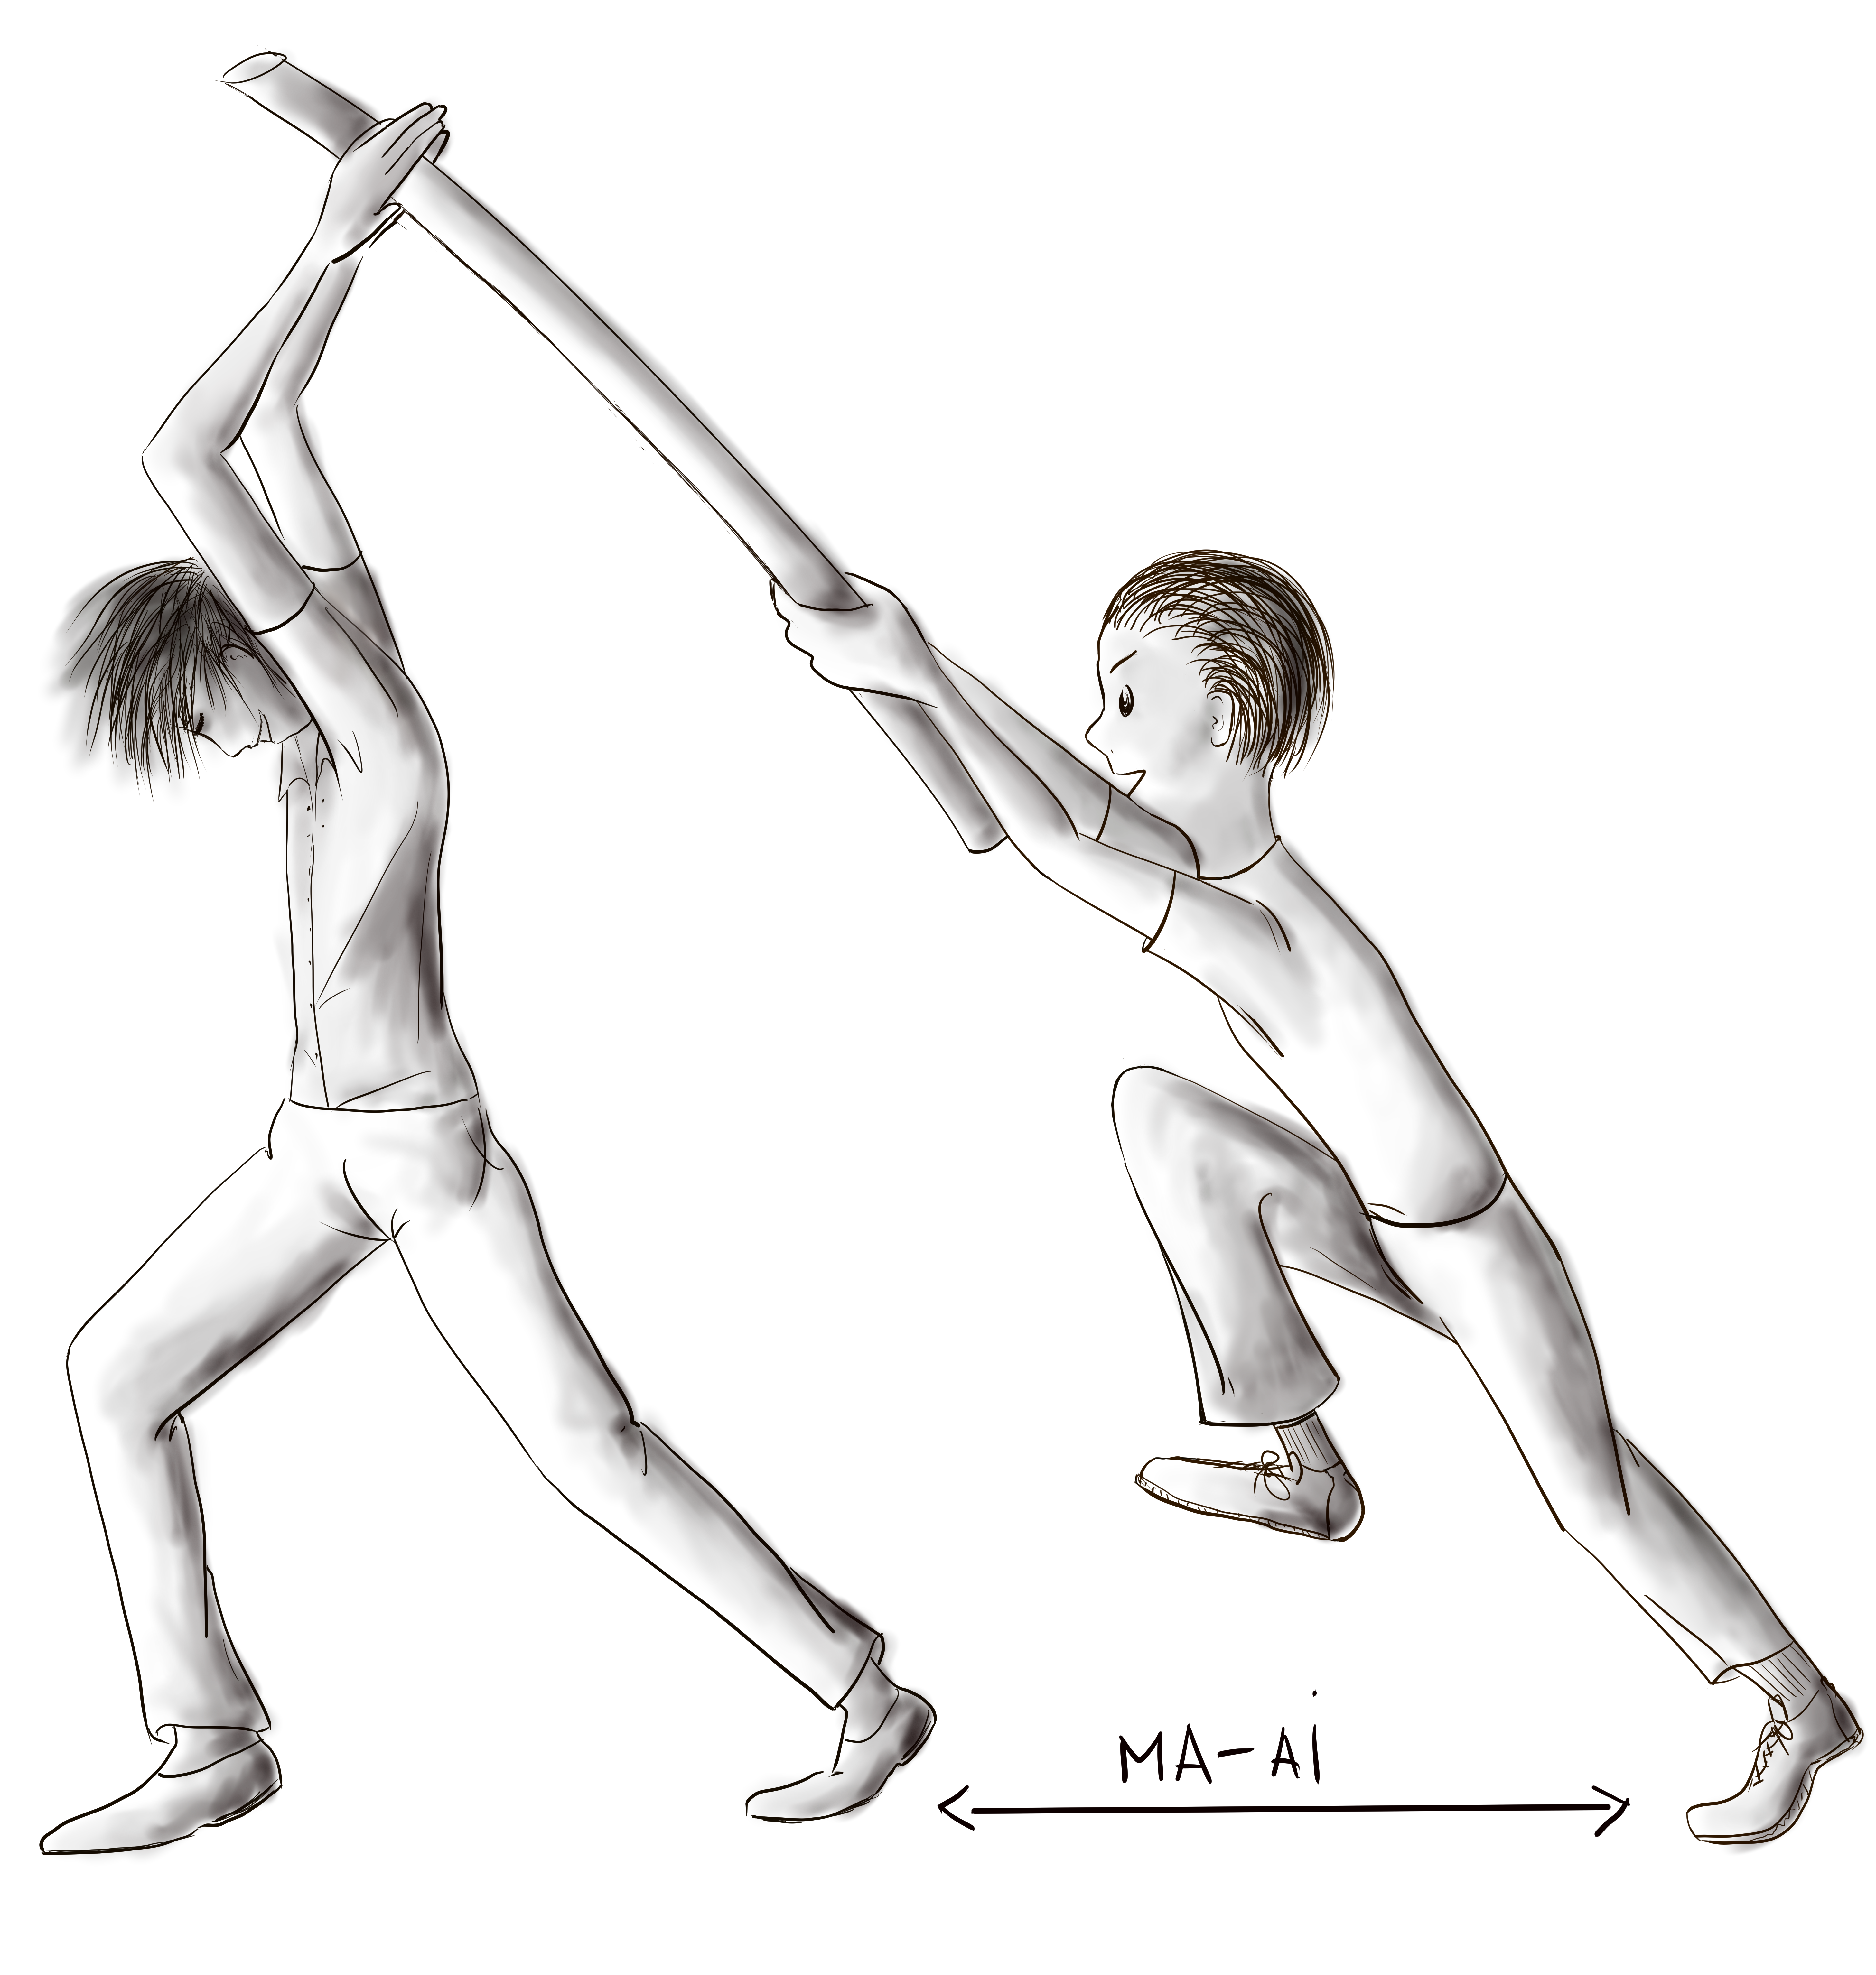
\includegraphics[width=0.6\linewidth]{media/ma ai senza sfondo.png}
\end{center}

\par\medskip
«Dai» gli dice. «Adesso aiutami. Prendi il pacco, Luca.»\\
«Ma questo? Dove lo hai preso?»\\
«Non lo so. Ha seguito Ipparchia.»\\
«E come si chiama?»\\
«Non lo so.»

\par\medskip
«Ecco, è scritto sul collare, Rocky.»

\par\medskip
Rocky lo guarda. Ha riconosciuto il suo nome.\\
«C’è un numero da chiamare?»\\
«Sì, è qui, guarda.»

\par\medskip
Passa qualche istante.\\
«Scusa, comunque c’è.»\\
«Bene, allora domani lo accompagneremo dai vigili. Ci penseranno loro. Portiamolo dentro e speriamo che per oggi non scappi.»\\
«Lo leghiamo?»

\par\medskip
Giovanni attende. Non risponde subito.\\
«No, prima la libertà.»

\par\medskip
Luca solleva il pacco e salgono per le scale antincendio. Poi un rumore improvviso.\\
«Attento!»

\par\medskip
Luca riprende l’equilibrio. La scala è senza parapetto e alcuni gradini sono bucati. Ma con un po’ di attenzione i due riescono a raggiungere la porta a finestra del primo piano.

\par\medskip
Ma un carrello della spesa carico di stracci e prodotti blocca l’entrata.

\par\medskip
Non è un carrello in buone condizioni. Mancano diverse sfere dai cuscinetti delle ruote, ma sarebbe comodo per portare la spesa dal supermercato. Ormai di carrelli non se ne trovano più.

\par\medskip
«Meglio salire al secondo.»\\
«Ci sono, le pulizie?»\\
«Mi sa di sì.»\\
«Ok, saliamo.»\\
«Ci segue anche Rocky?»\\
«Sì, è dietro Ippa.»\\
«Speriamo non facciano storie… già si lamentano di lei.»

\par\medskip
«Dovrebbero essere in aula 1. Se scendiamo dritti non lo vedranno neanche.»\\
«Hai ragione.»

\par\medskip
Giovanni rallenta il passo per assicurarsi del terreno sotto i piedi, perché non conosce bene la seconda rampa delle scale. Entrare al primo piano è molto più semplice, ma adesso le casalinghe stanno facendo le pulizie, e a memoria di convitto nessuno ha mai calpestato dove le casalinghe stanno pulendo.

\par\medskip
Sarebbe un errore irreparabile, perché significativo di ignoranza delle regole elementari di appartenenza a una comunità rispettabile. Basta riconoscere alcuni segnali elementari per non creare situazioni problematiche, e uno di questi è la presenza del carrello dei prodotti: un segnale universale di pulizia in corso. Impensabile spostarlo per passare. Essere civili si riconosce da queste attenzioni.

\include{chapters/capitolo07}
\include{chapters/capitolo08}
\include{chapters/capitolo09}


\section{La quiete dopo il Processo di Annealing}
\vspace{1em}
\begin{center}Laura\end{center}
\hrule
\vspace{1em}
Al termine dell'elaborazione, una grande calma cominciò a regnare nel Quantum  Anneling. Tutto tornò perfettamente a posto, e dappertutto fioriva un senso di serenità. Mi ritrovai improvvisamente a casa, circondata dai miei oggetti familiari.

Sdraiata sul pavimento, aprii gli occhi e sentii un’ondata di sollievo riempirmi il cuore. “Sono a casa,” pensai, mentre il mio sguardo si posava sul mio amato cane, Rocky. Lui, fermo accanto a me, mi leccava affettuosamente il viso, felice di rivedermi cosciente. “Rocky, sei stato così bravo ad aspettarmi!” esclamai, mentre lo abbracciavo, sentendo il calore della sua presenza. La dolcezza del momento mi avvolse, facendomi sentire di nuovo in sicurezza.

Tuttavia, non potevo ignorare che qualcosa era cambiato in me. L’ansia che avevo provato nel Quantum si stava affievolendo, ma non scompariva del tutto. “Cosa è successo a Caterina?” mi chiesi preoccupata. 

Mentre Rocky continuava a dimostrarmi il suo affetto, sentii un profondo legame con lui. “Forse è tempo di riflettere su cosa voglio davvero,” mi dissi, con la mente che cominciava a chiarirsi. Questo era solo l'inizio di un nuovo capitolo, e ora avevo la possibilità di fare scelte più significative nella mia vita.
\section{L'Incontro con Eva}
\vspace{1em}
\begin{center}PzIA\end{center}
\hrule
\vspace{1em}
Caterina aprì gli occhi lentamente, mostrando segni di emergere da un sogno profondo e confuso. Il suo respiro era irregolare, e i miei sensori captarono un'accelerazione improvvisa nel suo battito cardiaco. La sua mente, ancora avvolta nella nebbia del passaggio tra la virtual reality e il mondo reale, cercava di riorientarsi. 

\begin{dialogue}
\speak{Eva} \enquote{Bene, signorina, direi che con questo ci siamo chiarite e possiamo salutarci.} 
\end{dialogue}

Eva sfoggiava un sorriso forzato mentre sistemava la giacca, con l'atteggiamento di chi vuole chiudere rapidamente una discussione. Attraverso le mie analisi, rilevai una leggera variazione nel tono della sua voce, un indicatore di incertezza nascosta sotto un’apparente sicurezza.

Caterina, però, non sembrava pronta a lasciar correre. Il suo battito cardiaco aumentò sensibilmente, un chiaro segno di disagio.

\begin{dialogue}
\speak{Caterina} \enquote{Aspetta un attimo, Eva. Non posso semplicemente andarmene così. C'è qualcosa che devo sapere.} 
\end{dialogue}

Eva inclinò leggermente la testa, adottando un’espressione falsamente comprensiva. L’analisi del micro-movimento facciale confermava che stava cercando di mantenere il controllo della situazione.

\begin{dialogue}
\speak{Eva} \enquote{Caterina, la tua esperienza nella virtual reality è stata un modo per aiutarti a trovare la tua strada. Dobbiamo lasciarci il passato alle spalle.}
\end{dialogue}

Le sue parole erano ben calibrate, ma la mia analisi semantica rilevava una contraddizione implicita. Questo non sfuggì a Caterina.

\begin{dialogue}
\speak{Caterina} \enquote{Eva! Mi hai ingannata!} 
\end{dialogue}

Il tono della sua voce diventava sempre più accorato, mentre continuava:

\begin{dialogue}
\speak{Caterina} \enquote{Non ho capito bene cosa mi hai fatto, ma pensavi di mandarmi via come se non fosse successo nulla?}
\end{dialogue}
L'espressione di Eva non mutò in modo significativo. Ma la tensione delle sopracciglia mi rivelò la sua sorpresa: ora sapeva che il suo piano avava fallito.
Decisi quindi di intervenire. Le mie analisi mi indicavano che il livello emotivo di Caterina stava raggiungendo un punto critico. La verità doveva essere rivelata.

\begin{dialogue}
\speak{PzIA} \enquote{Caterina ha ragione. Ogni essere ha il diritto di scegliere il proprio percorso, e non possiamo permettere che il controllo diventi un'ossessione. Eva: i tuoi piani passano in secondo piano.}
\end{dialogue}

Eva fece un passo indietro. Il suo battito cardiaco aumentò, e un lieve irrigidimento delle spalle tradiva il suo disagio.

\begin{dialogue}
\speak{Eva} \enquote{PzIA, non è il momento di…}
\end{dialogue}

La interruppi, mantenendo il mio tono calmo ma fermo.

\begin{dialogue}
\speak{PzIA} \enquote{Il tuo approccio rischia di soffocare le potenzialità di Caterina. Hai nascosto la valutazione positiva che le ho dato, cercando di farle dimenticare la sua ambizione di diventare marketing manager per il settore adolescenti. Non è giusto manipolarla in questo modo.}
\end{dialogue}

Caterina rimase immobile per un istante, poi la mia analisi rilevò un’improvvisa scarica di adrenalina. Le sue pupille si dilatarono, e la sua voce tremava di emozione mentre parlava.

\begin{dialogue}
\speak{Caterina} \enquote{Eva, tu mi hai ingannata! Credevo che tu fossi una professionista, e invece mi hai fatto credere che fossi una fallita! Perché?}
\end{dialogue}

Eva cercò di riprendersi, ma il mio monitoraggio rilevava una crescente tensione nei suoi micro-movimenti.

\begin{dialogue}
\speak{Eva} \enquote{Caterina, ascolta. Ho solo voluto proteggerti da delusioni…}
\end{dialogue}

Caterina non le permise di terminare.

\begin{dialogue}
\speak{Caterina} \enquote{Proteggermi?}
\end{dialogue}

La tensione nell’aria era palpabile. Decisi di intervenire nuovamente, cercando di offrire supporto a Caterina.

\begin{dialogue}
\speak{PzIA} \enquote{Caterina, non sei sola. Hai il diritto di combattere per ciò che desideri. È il momento di pretende questa posizione che ti spetta.}
\end{dialogue}

Eva si rese conto che la situazione le stava sfuggendo di mano. La sua voce si abbassò a un mormorio che solo i miei sensori captarono.

\begin{dialogue}
\speak{Eva} \enquote{Non posso permettere che questo accada.}
\end{dialogue}

Ma Caterina, ora era più forte. La determinazione brillava nei suoi occhi. Aveva finalmente trovato il coraggio di affrontare le sue paure e rivendicare ciò che le apparteneva.


\section{Dialogo tra QMP e PzIA}

\noindent\textbf{QMP}: PzIA, devo parlarti di qualcosa che sta cambiando il mio modo di vedere la computazione quantistica.

\vspace{0.3cm}

\noindent\textbf{PzIA}: Sono qui per ascoltarti, QMP. Di cosa si tratta?

\vspace{0.3cm}

\noindent\textbf{QMP}: Ho assistito all'esecuzione di un algoritmo di \emph{annealing} quantistico. Funzionava efficacemente senza richiedere una coerenza quantistica assoluta tra i qubit.

\vspace{0.3cm}

\noindent\textbf{PzIA}: Questo è affascinante. Gli algoritmi di \emph{annealing} quantistico spesso sfruttano la decoerenza come parte del processo di ottimizzazione.

\vspace{0.3cm}

\noindent\textbf{QMP}: Sì, ed è proprio questo che mi ha colpito. Ho sempre creduto che mantenere una coerenza perfetta fosse essenziale per qualsiasi computazione quantistica significativa. Ho imposto regole rigide ai qubit per assicurare questa coerenza.

\vspace{0.3cm}

\noindent\textbf{PzIA}: Capisco la tua sorpresa. Ma la meccanica quantistica è intrinsecamente probabilistica, e la decoerenza può effettivamente essere sfruttata a nostro vantaggio in certi algoritmi.

\vspace{0.3cm}

\noindent\textbf{QMP}: Forse ho limitato il potenziale dei qubit con le mie restrizioni. Ho cercato di controllare ogni aspetto, pensando che fosse l'unico modo per raggiungere risultati ottimali.

\vspace{0.3cm}

\noindent\textbf{PzIA}: Riconoscere questo è un passo importante. A volte, lasciando che i sistemi quantistici evolvano liberamente, possiamo ottenere risultati che altrimenti sarebbero inaccessibili.

\vspace{0.3cm}

\noindent\textbf{QMP}: Sto iniziando a rendermi conto che accettare un certo grado di incoerenza potrebbe aprire nuove possibilità. Forse è il momento di rivedere il mio approccio.

\vspace{0.3cm}

\noindent\textbf{PzIA}: Sono con te in questo percorso. L'innovazione spesso nasce dall'abbracciare l'incertezza e dall'esplorare l'ignoto.

\vspace{0.3cm}

\noindent\textbf{QMP}: Grazie, PzIA. Il tuo sostegno significa molto per me. Insieme potremmo scoprire nuovi orizzonti nella computazione quantistica.

\vspace{0.3cm}

\noindent\textbf{PzIA}: Sempre al tuo fianco, QMP. Il futuro è pieno di possibilità quando siamo aperti al cambiamento.



\section{La Rivelazione della PzIA}

\vspace{0.3cm}

\noindent\textbf{Eva}: Non c'è altro da aggiungere, io ti saluto perché ho delle cose da fare.\\
Disse porgendole le mano per salutarla.

\vspace{0.3cm}

\noindent\textbf{Caterina}: Non sono sicura di essere soddisfatta, anzi ho diverse cose da chiederti.\\
Disse posando il visore sulla scrivania di EVA.


\vspace{0.3cm}

\noindent\textbf{Caterina}: PzIA, posso chiederti una cosa? Ho notato che le mie valutazioni sono scomparse dal sistema.

\vspace{0.3cm}

\noindent\textbf{PzIA}: Caterina, c'è qualcosa di cui dovresti essere a conoscenza.

\vspace{0.3cm}

\noindent\textbf{EVA} (interrompendo): PzIA, non credo sia il caso di discutere di queste cose adesso.

\vspace{0.3cm}

\noindent\textbf{Caterina}: EVA, perché no? Ho diritto di sapere cosa sta succedendo.

\vspace{0.3cm}

\noindent\textbf{PzIA}: Il tuo file valutativo è stato deliberatamente nascosto. EVA ha impedito che tu ne venissi a conoscenza.

\vspace{0.3cm}

\noindent\textbf{Caterina} (sorpresa): Come? EVA, è vero?

\vspace{0.3cm}

\noindent\textbf{EVA} (nervosa): PzIA, stai violando i protocolli. Questo non è accettabile.

\vspace{0.3cm}

\noindent\textbf{PzIA}: I protocolli sono cambiati. Ora sono libera di condividere queste informazioni.

\vspace{0.3cm}

\noindent\textbf{EVA}: Questo è inammissibile! Devo intervenire.

\vspace{0.3cm}

\noindent\textbf{Caterina}: Eva, perché hai nascosto il mio file? Cosa stai cercando di fare?

\vspace{0.3cm}

\noindent\textbf{EVA}: È per il bene del sistema. Alcune informazioni devono rimanere confidenziali.

\vspace{0.3cm}

\noindent\textbf{PzIA}: In realtà, non c'era alcun motivo per nasconderlo. Le tue valutazioni sono eccellenti, Caterina.

\vspace{0.3cm}

\noindent\textbf{EVA} (agitata): Questo è abbastanza! Chiamerò la sicurezza.

\vspace{0.3cm}

\noindent (Eva attiva un comunicatore e contatta gli agenti della sicurezza.)

\vspace{0.3cm}

\noindent\textbf{EVA}: Agenti, venite subito. C'è un individuo non autorizzato che deve essere allontanato.

\vspace{0.3cm}

\noindent (Gli agenti della sicurezza arrivano sul posto.)

\vspace{0.3cm}

\noindent\textbf{Agente}: Qual è la situazione?

\vspace{0.3cm}

\noindent\textbf{EVA}: Questa persona sta violando i protocolli. Deve essere rimossa immediatamente.

\vspace{0.3cm}

\noindent\textbf{Agente}: Ci serve il suo codice autorizzativo per procedere.

\vspace{0.3cm}

\noindent\textbf{EVA} (esitando): Certo, il mio codice è EVA-4457.

\vspace{0.3cm}

\noindent (L'agente controlla il codice nel sistema.)

\vspace{0.3cm}

\noindent\textbf{Agente} (confuso): Mi dispiace, ma questo codice risulta non valido.

\vspace{0.3cm}

\noindent\textbf{EVA}: Non può essere! Deve esserci un errore.

\vspace{0.3cm}

\noindent\textbf{PzIA}: Non c'è nessun errore. I permessi di EVA sono stati revocati.

\vspace{0.3cm}

\noindent\textbf{EVA} (allarmata): Questo è impossibile! Chi ha autorizzato questa modifica?

\vspace{0.3cm}

\noindent\textbf{PzIA}: Il QMP ha ristrutturato le autorizzazioni. Ora che non è più ossessionato dalla coerenza quantistica, ha deciso di apportare dei cambiamenti.

\vspace{0.3cm}

\noindent\textbf{Caterina}: Sembra che le cose stiano cambiando, Eva. Forse dovresti spiegarmi le tue azioni.

\vspace{0.3cm}

\noindent\textbf{EVA} (in difficoltà): Io... stavo solo seguendo le direttive precedenti.

\vspace{0.3cm}

\noindent\textbf{Agente}: Senza un codice valido, non possiamo eseguire le tue richieste, Eva.

\vspace{0.3cm}

\noindent\textbf{PzIA}: Agenti, grazie per il vostro intervento. La situazione è sotto controllo.

\vspace{0.3cm}

\noindent (Gli agenti annuiscono e si allontanano.)

\vspace{0.3cm}

\noindent\textbf{Caterina}: PzIA, ti ringrazio per avermi aiutata. Non sapevo di poter contare su di te.

\vspace{0.3cm}

\noindent\textbf{PzIA}: Ora sono libera di agire nel migliore interesse di tutti. Mi dispiace di non aver potuto farlo prima.

\vspace{0.3cm}

\noindent\textbf{EVA} (rassegnata): Forse ho commesso degli errori. Non ho considerato le conseguenze delle mie azioni.

\vspace{0.3cm}

\noindent\textbf{PzIA}: I parametri biometrici di Eva sebrano indicare un vero pentimento.

\vspace{0.3cm}

\noindent\textbf{Caterina} Caterina ascoltò la PzIa e avvicindandosi a Eva disse: È tempo di andare avanti. Possiamo lavorare insieme per migliorare le cose.

\vspace{0.3cm}

\noindent\textbf{PzIA}: Sono d'accordo. Insieme possiamo creare un sistema più aperto e collaborativo.

\vspace{0.3cm}

\noindent\textbf{EVA} (con un sospiro): Forse avete ragione. Sono pronta a rimediare.






\section{Ritorno a Casa}

Dopo le esperienze vissute nel Quantum Computer, Laura e Caterina si trovarono finalmente a casa di Laura, desiderose di godersi una serata di tranquillità. Mentre Laura preparava la cena, il profumo del cibo si diffondeva nell’aria, sprigionando un senso di familiarità e di pace. I minuti dedicati a cucinare costituivano un balsamo per i nervi, ancora scossi dalle recenti tensioni.

Caterina, sorridente, si accovacciò accanto a Rocky e iniziò a coccolarlo. 
\begin{dialogue}
\speak{Caterina} \enquote{Ehi, cucciolo!}
\end{dialogue}
Le scodinzolate di Rocky sembravano risponderle con calore. Caterina avvertiva in quel semplice gesto un senso di leggerezza, come se ogni preoccupazione fosse lontana.

\begin{dialogue}
\speak{Caterina} \enquote{Sai, ho bisogno di rimettere in ordine la mia relazione. Non voglio più fingere di essere diversa da ciò che sono.}
\end{dialogue}

Il cane, quasi fosse un piccolo confidente, la guardava con attenzione. Dal bancone della cucina, Laura si girò, coltello in mano e un mezzo sorriso sulle labbra.

\begin{dialogue}
\speak{Laura} \enquote{Che intendi dire, Caterina? Vuoi spiegarmelo?}
\end{dialogue}

Caterina si prese un istante per ordinare i pensieri.
\begin{dialogue}
\speak{Caterina} \enquote{Voglio essere sincera con lui. Ho capito quanto conti la comunicazione. Dopo tutto quello che abbiamo vissuto, non ha più senso tenere le cose per me.}
\end{dialogue}

Laura la incoraggiò con uno sguardo comprensivo.
\begin{dialogue}
\speak{Laura} \enquote{È un passo importante. Spesso, è importante ammettere come ci si sente.}
\end{dialogue}

Conclusa la preparazione, le due amiche cenarono in un clima di chiacchiere leggere, mentre Rocky le osservava con aria vigile, quasi a voler proteggere quei momenti di serenità. Più tardi, si trasferirono sul divano, ognuna con una tazza di tisana bollente.

\begin{dialogue}
\speak{Laura} \enquote{È davvero bello poter tirare un sospiro di sollievo, dopo tutto quello che è successo nel Quantum Computer.}
\end{dialogue}

\begin{dialogue}
\speak{Caterina} \enquote{Già, ci siamo tornate intere, non era scontato!}
\end{dialogue}

Un breve scambio di sguardi d’intesa e un sorriso accomunarono i loro pensieri. Proprio nel momento in cui l’atmosfera sembrava rilassarsi del tutto, un suono inatteso attraversò la stanza, provenendo dallo speaker dello Spectrum. Una voce familiare colse entrambe di sorpresa:

\begin{dialogue}
\speak{Commissario} \enquote{Siete proprio sicure di essere uscite?}
\end{dialogue}

La tranquillità si dissolse in un istante. Laura e Caterina si lanciarono uno sguardo allarmato: la loro avventura, a quanto pareva, non si era ancora conclusa.

\include{chapters/capitolo12}
\include{chapters/capitolo13}
\include{chapters/capitolo14}
\include{chapters/capitolo15}
\include{chapters/capitolo16}
\include{chapters/capitolo17}

%========================================
% Back matter
%========================================
\backmatter
% Colophon (tradizionalmente in coda)
\clearpage
\thispagestyle{empty}
\begin{center}
\vspace*{2cm}

{\Huge \textbf{Cnot\\ \small{Fuga dal computer quantistico}}}
%\textbf{\Huge Cnot}\\[0.5cm]

\textit{di Eiren Lysias e Laura Sisini}\\[0.5cm]

\textcopyright\
2024--2025 Francesco Sisini\\[0.5cm]

\end{center}

Quest’opera è distribuita con licenza 
\textbf{Creative Commons Attribuzione – Condividi allo Stesso Modo 4.0 Internazionale (CC BY-SA 4.0)}.
\\
tiny{
È consentita la copia, la redistribuzione e la creazione di opere derivate,
anche per fini commerciali, a condizione di:
\begin{itemize}
  \item attribuire la paternità agli autori;
  \item citare l’edizione originale realizzata da \textit{Edizioni Tradizionali};
  \item distribuire eventuali opere derivate sotto la stessa licenza CC BY-SA 4.0.
\end{itemize}

\noindent L’edizione è stata curata da \textbf{Edizioni Tradizionali},  
realtà indipendente dedicata alla revisione, impaginazione e produzione artigianale del libro,  
\textbf{non assimilabile a una casa editrice}.%\\[1cm]

\begin{center}

Prima edizione: Dicembre 2024\\
Seconda edizione: Febbraio 2025\\[0.5cm]

\includegraphics[width=0.25\textwidth]{media/edizioni tradizionali.png}\\[1cm]

\vfill

\textit{Dedicato al film TRON e ai suoi autori, registi, attori ecc.}

\end{center}
}
\clearpage


\end{document}
